\subsection{Methodology}


We propose a methodology to demystify GPU microarchitecture features and correlate them with microbenchmarks' performance.
The workflow in Figure~\ref{fig:workflow} consists of three major components: a GPU ISA encoding solver, a GPU assembler, and the meticulous benchmarking.
A sample program in Figure~\ref{fig:workflow} is a synthetic PTX file which generates specific instructions as the input of the instruction solver.
Deliberate microbenchmarks are designed for our assembler to tune code at assembly language level and used to figure out the correlation between microarchitecture and performance.
%We dissemble a binary library (such as cuBLAS) to provide a high coverage of instructions to instruction solver.
%We use cuBLAS in this work since it contains nearly all needed instructions for SGEMM routine.


We write a simple generator to produce PTX instructions with various modifiers as the PTX samples.
% We first leverage CUDA binary tools ({\tt cuobjdump} and {\tt nvdisasm}) to disassemble {\tt cubin} generated by sample programs. 
PTX files are compiled to {\tt cubin} files by {\tt ptxas}, and then disassembled by {\tt cuobjdump} to generate their native assemblies. 
The ISA encoding solver takes the assembly files {\em sass}) as the input to decode each field of 64-bit instructions.
A set of algorithms are designed to solve all fields, {\em operands}, {\em opcodes}, and {\em modifiers}, of a binary instruction.
{\tt cuobjdump} and {\tt nvdisasm} are also used to disassemble temporary instructions generated from the solver algorithms.
%The solver uncovers some undocumented ISA specifications,
%which is used to implement an naive assembler.
Our assembler translates every instruction field to get 64-bit binaries and then encapsulates them with an ELF header to generate an executable cubin file.
% which can be used by CUDA driver APIs.
\jli{describe microbenchmark: one sentence}
In the benchmarking workflow (red arrows in Figure~\ref{fig:workflow}), assembly microbenchmarks are tuned to explore GPU architecture features such as register bank, instruction throughput, control codes, and load/store width.
% In the end, the tuning process will lead to some practical observations on the correlation between microarchitecture and performance.


\begin{figure}[htbp]
\begin{center}
    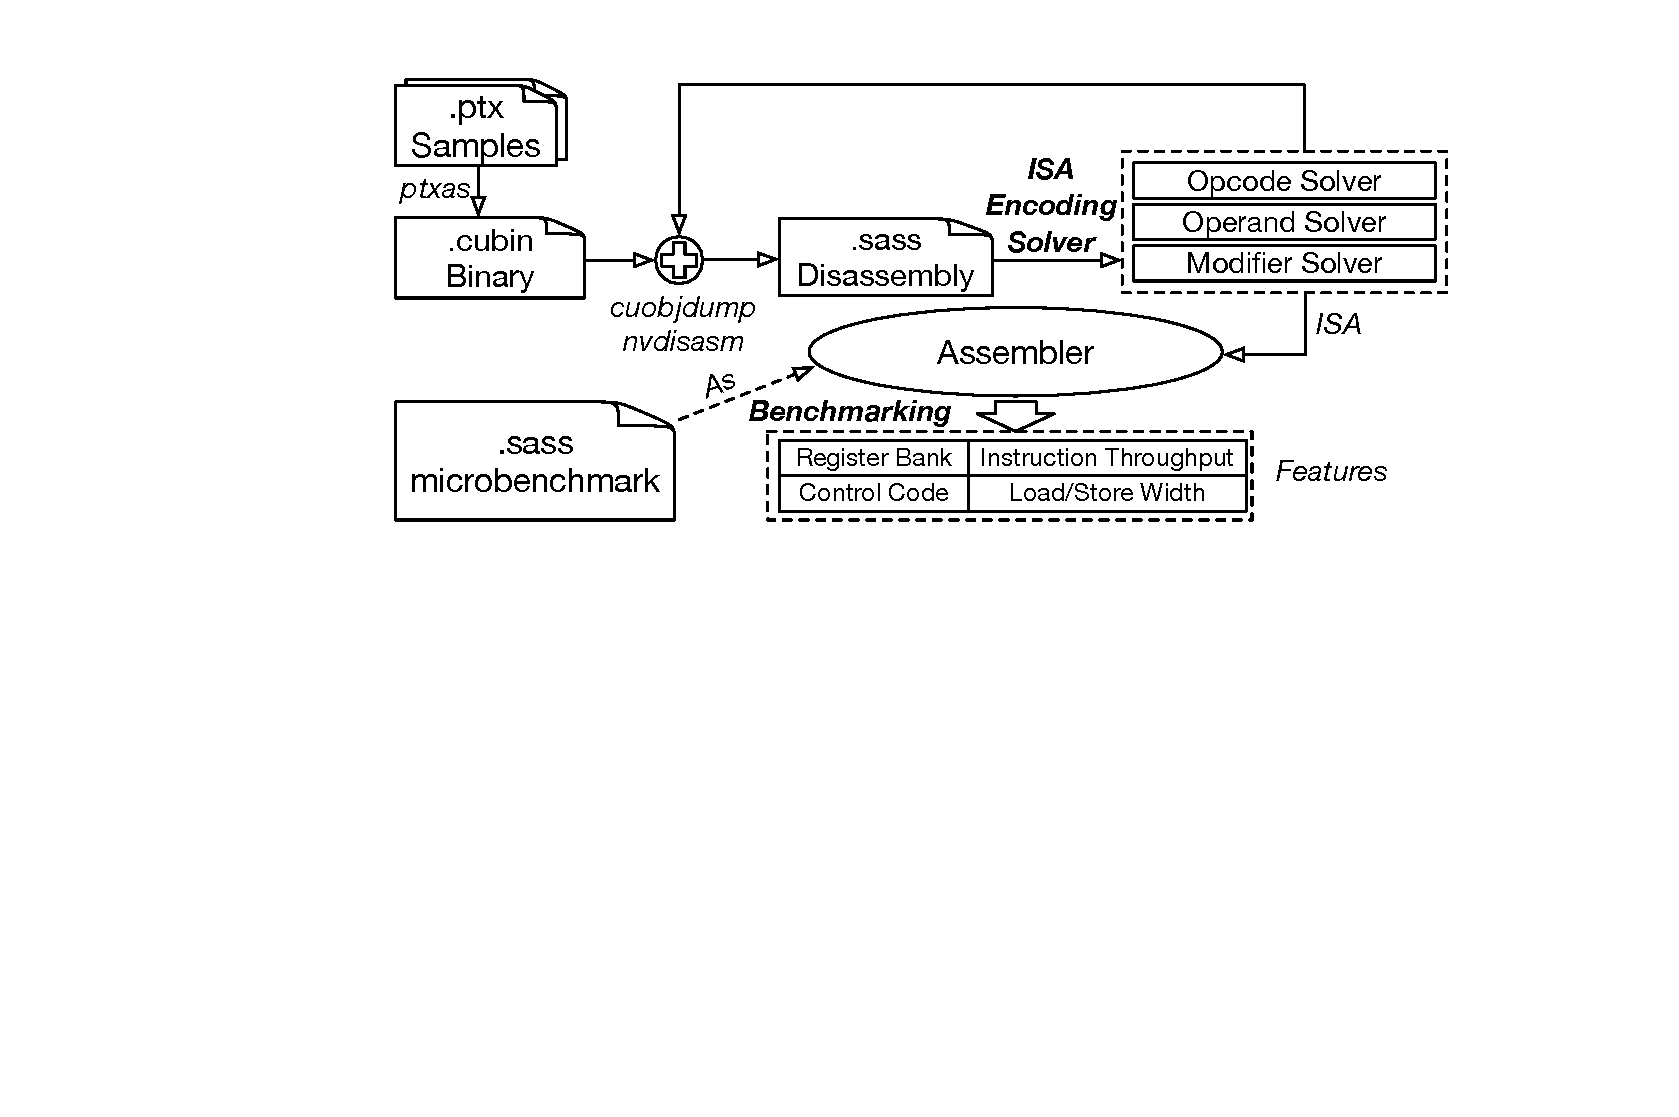
\includegraphics[scale=0.4]{methodology_new}
\caption{A schematic diagram of demystifying GPU microarchitecture features by leveraging CUDA binary tools. The black arrows
    represent the workflow of instruction solver while the red ones represents benchmarking to find out the correlation between microarchitecture and performance.}
\label{fig:workflow}
\end{center}
\end{figure}
